\section{Rechnung an einem Konkreten Beispiels}

\subsection{Brechungsgesetz von Snellius \label{brechungsgesetz}}
\cite{Wikipedia} Aus dem Fermatschen Prinzip lässt sich das Brechungsgesetz von Snellius herleiten.
Das Licht legt den Weg vom Startpunkt $P_0$ über den Brechungspunkt $P_1$ 
nach dem Endpunkt $P_2$ zurück, siehe \figref{Ab:brechung}.
\begin{figure}[H]
	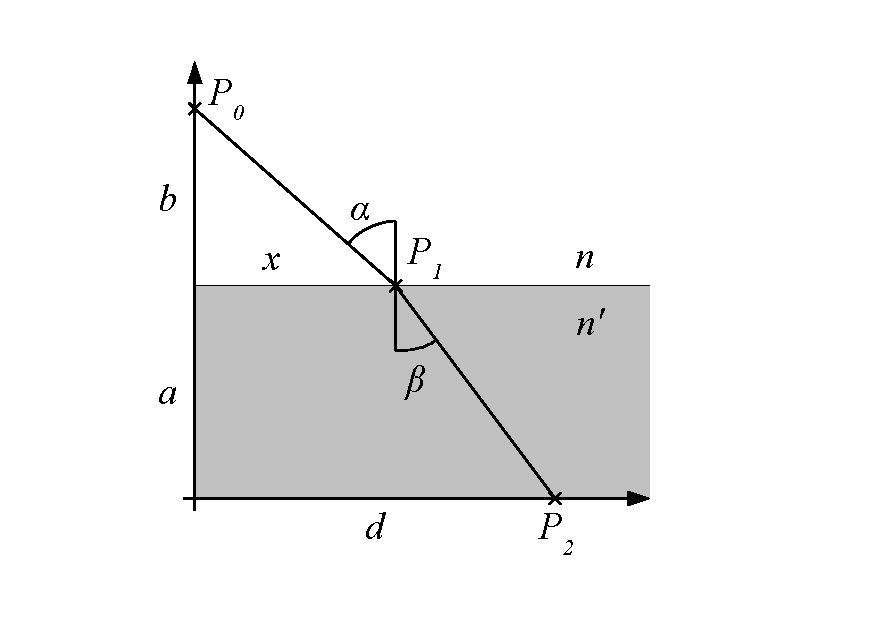
\includegraphics[width=0.8\textwidth]{./picture/Brechung.pdf}
	\caption{Skizze des Brechungsgesetzes von Snellius}
	\label{Ab:brechung}
\end{figure}

Dadurch kann die zurückgelegte Zeit berechnet werden, siehe \eqref{snelliusT}.
\begin{align}
t(x) = t_1 + t_2 = \frac{s_1}{c_1} + \frac{s_2}{c_2} = \frac{|P_1 - P_0|}{c_1} + \frac{|P_2 - P_1|}{c_2} \notag \\
= \frac{\sqrt{a^2 + x^2}}{c_1} + \frac{\sqrt{(d-x)^2 + b^2}}{c_2} \label{snelliusT}
\end{align}

Leiten wir diese Funktion nun nach $dx$ ab, finden wir eine \texttodo{die ? Extrem....} Extremastelle von $t$, siehe \eqref{snelliusDx}.
\begin{align}
	\frac{dt}{dx} = \frac{2 \cdot x}{2 \cdot c_1 \cdot \sqrt{a^2 + x^2}} + \frac{-2 \cdot (d-x)}{2 \cdot c_2 \cdot \sqrt{(d-x)^2 + b^2}} = \notag \\
	\frac{x}{c_1 \cdot \sqrt{a^2 + x^2}} - \frac{(d-x)}{c_2 \cdot \sqrt{(d-x)^2 + b^2}} = 0 \label{snelliusDx}
\end{align}

Aus \figref{Ab:brechung} ist gut ersichtlich das folgende Substitutionen \ref{substitution} durchgeführt werden können

\begin{align}
	x = \sin(\alpha) \cdot \sqrt{a^2 + x^2} \notag \\
	d-x = \sin(\beta) \cdot \sqrt{(d -x)^2 + b^2} \label{substitution}
\end{align}


\texttodo{sehr grosser sprung, aufwändig zum nachvollziehen, zwischenschritte einfügen}
daraus ergibt sich das Verhältnis gemäss \eqref{snellius}.
\begin{equation}
	0 = \frac{\sin(\alpha)}{c_1} - \frac{\sin(\beta)}{c_2} \Leftrightarrow\frac{c_2}{c_1} = \frac{\sin(\beta)}{\sin(\alpha)}
	\label{snellius}
\end{equation}


%Diese Funktion bis jetzt ist ja schön und gut, 
%jedoch konnte noch nicht nachgewiesen werden, 
%dass die Extremalstelle auch wirklich ein Minimum ist. 
%Deshalb müssen wir nun noch die zweite Ableitung berechnen.

%\[
%0 > 
%\frac{dt^2}{d^2x} \left(\frac{\sqrt{a^2 + x^2}}{c_1} + 
%\frac{\sqrt{(d-x)^2 + b^2}}{c_2}\right) =
%\frac{dt}{dx} \left(\frac{x}{c_1 \cdot \sqrt{a^2 + x^2}} - 
%\frac{(d-x)}{c_2 \cdot \sqrt{(d-x)^2 + b^2}} \right) = \phantom a
%\]
%\[
%- \frac{x^2}{c_1 \cdot \sqrt{(a^2 + x^2)}^{3}}
%+ \frac{1}{c_1 \cdot \sqrt{a^2 + x^2}}
%+ \frac{(d-x)\cdot(x-d)}{c_2 \cdot \sqrt{(b^2 + (d - x)^2)}^{3}}
%+ \frac{1}{c_2 \cdot \sqrt{b^2 + (d-x)^2}} = \phantom a
%\]
%\[
%\frac{a^2}{c_1 \cdot \sqrt{(a^2 + x^2)}^{3}}
%+ \frac{b^2}{c_2 \cdot \sqrt{(b^2 + (d - x)^2)}^{3}} = \phantom a
%\]

\subsection{Reflexionsgesetz}
\cite{Wikipedia} Auf gleiche weise wie das das Brechungsesetz aus dem Fermatschen Prinzip hergeleitet wird, 
lässt sich daraus auch das Reflexionsgesetz ableiten.
Das Licht legt den Weg vom Startpunkt $P_0$ über den Spiegelpunkt $P_1$ 
nach dem Endpunkt $P_2$ zurück. Dadurch kann die zurückgelegte Zeit berechnet werden, siehe \eqref{reflexion}.



\begin{align}
t(x) = t_1 + t_2 = \frac{s_1 + s_2}{c} = \frac{|P_1 - P_0| + |P_2 - P_1|}{c} \notag \\
= \frac{\sqrt{a^2 + x^2} + \sqrt{(d-x)^2 + b^2}}{c} \label{reflexion}
\end{align}

$t(x)$ nach $dx$ abgeleitet ergibt eine Extremalstelle  von $t$, siehe \eqref{reflexionDx}.

\begin{align}
\frac{dt}{dx} = \frac{1}{c} \cdot \frac{2 \cdot x}{2 \cdot \sqrt{a^2 + x^2}} + \frac{-2 \cdot (d-x)}{2 \cdot \sqrt{(d-x)^2 + b^2}} \notag \\
= \frac{x}{ \sqrt{a^2 + x^2}} - \frac{(d-x)}{ \sqrt{(d-x)^2 + b^2}} \label{reflexionDx}
\end{align}

\begin{figure}[H]
	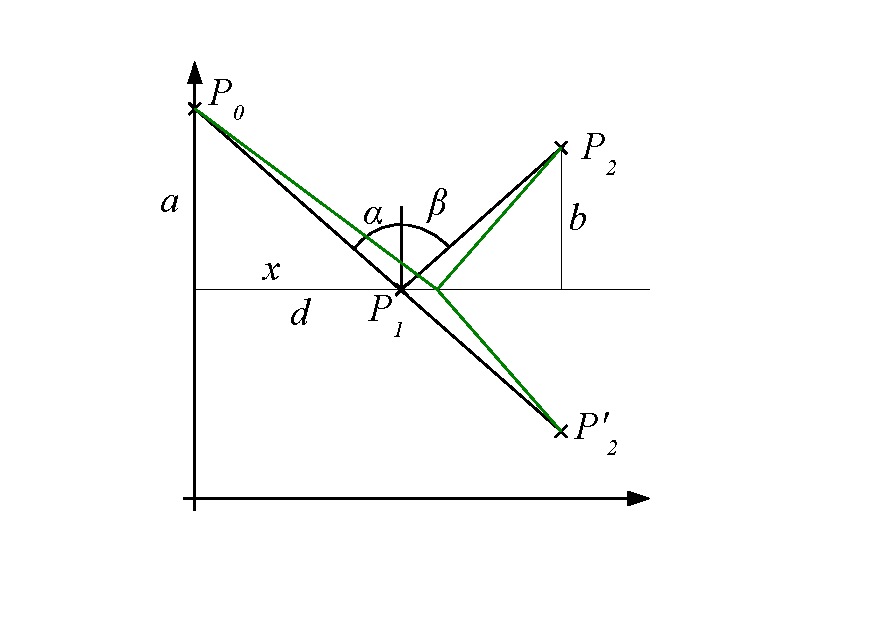
\includegraphics[width=0.8\textwidth]{./picture/Spiegelung.pdf}
	\caption{Skizze des Reflexionsgesetzes}
	\label{Ab:spiegelung}
\end{figure}

Aus \figref{Ab:spiegelung} ist gut ersichtlich das die Substitution \ref{substitution}  von \secref{brechungsgesetz} auch hier nützlich ist.


\texttodo{sehr grosser sprung, aufwändig zum nachvollziehen, zwischenschritte einfügen}
daraus ergibt sich das Eintritts- und Austrittswinkel gleich sind, siehe \eqref{brechung}.


\begin{equation}
0 = \sin(\alpha) - \sin(\beta) \Leftrightarrow \sin(\beta) = \sin(\alpha) \Leftrightarrow\beta = \alpha
\end{equation}

In \figref{Ab:spiegelung} ist ersichtlich, dass die Linie des Startpunktes bis zum 
gespiegelten Endpunkt eine Gerade ist, welche der Funktion des kürzesten Weges entspricht.

%Diese Funktion bis jetzt ist ja schön und gut, 
%jedoch konnte noch nicht nachgewiesen werden, 
%dass die Extremalstelle auch wirklich ein Minimum ist. 
%Deshalb müssen wir nun noch die zweite Ableitung berechnen.

%\[
%0 > 
%\frac{dt^2}{d^2x} \left(\frac{\sqrt{a^2 + x^2}}{c_1} + 
%\frac{\sqrt{(d-x)^2 + b^2}}{c_2}\right) =
%\frac{dt}{dx} \left(\frac{x}{c_1 \cdot \sqrt{a^2 + x^2}} - 
%\frac{(d-x)}{c_2 \cdot \sqrt{(d-x)^2 + b^2}} \right) = \phantom a
%\]
%\[
%- \frac{x^2}{c_1 \cdot \sqrt{(a^2 + x^2)}^{3}}
%+ \frac{1}{c_1 \cdot \sqrt{a^2 + x^2}}
%+ \frac{(d-x)\cdot(x-d)}{c_2 \cdot \sqrt{(b^2 + (d - x)^2)}^{3}}
%+ \frac{1}{c_2 \cdot \sqrt{b^2 + (d-x)^2}} = \phantom a
%\]
%\[
%\frac{a^2}{c_1 \cdot \sqrt{(a^2 + x^2)}^{3}}
%+ \frac{b^2}{c_2 \cdot \sqrt{(b^2 + (d - x)^2)}^{3}} = \phantom a
%\]

\subsection{Fata Morgana Allgemein}

Bei einer Fata Morgana hat die Luft eine optische Dichte von $n(x,y)$. 
Dabei bewegt sich das Licht mit der Geschwindigkeit $c/n(x,y)$. 
Die benötigte Zeit, damit das Licht vom Punkt $(x_0, y_0)$ nach $(x_1, y_1)$ braucht,
kann mit dem Kurvenintegral berechnet werden.

\begin{equation}
T(y) = \int \limits_{x_0}^{x_1} \frac{n(x,y)}{c} \sqrt{1 + y'(x)^2} dx
\end{equation}

Wie es bei einem heissen Tag auf einer Strasse oder in einer Wüste zutrifft,
nehmen wir zuerst nur einmal an, dass die optische Dicht nur von $y$ abhängt
(also $n(x,y) = g(y)$) und mit zunehmenden $y$ ebenfalls zunimmt. 
Mathematisch bedeuted dies:

\begin{equation}
g(y) > 0 
\end{equation}

\begin{equation}
g'(y) > 0
\end{equation}

Dieses Minimalproblem zu lösen, wird die Euler-Lagrange-Gleichung des Variationsproblems

\begin{equation}
T(y) = \int \limits_{x_0}^{x_1} \frac{g(y)}{c} \sqrt{1 + y'(x)^2} dx = \frac{1}{c} \int \limits_{x_0}^{x_1} g(y) \sqrt{1 + y'(x)^2} dx
\end{equation}

aufgestellt. Der Faktor $\frac{1}{c}$ keinen Einfluss auf das Integral und 
somit auf das Variationproblem hat 
und er nur ständig mitgeschleppt werden würde, lassen wir ihn weg.
Es werden nun die Ableitungen der Funktion 

\begin{equation}
F(x,y,y') = g(y) \sqrt{1 + y'^2}
\end{equation}

gebraucht und lauten:

\begin{equation}
\frac{\partial F}{\partial y} = g'(y) \sqrt{1 + y'^2}
\end{equation}

\begin{equation}
\frac{\partial F}{\partial y'} = g(y) \frac{y'}{\sqrt{1 + y'^2}}
\end{equation}

Für die Euler-Lagrange-Gleichung muss man im zweiten Ausdruck $y(x)$ 
und $y'(x)$ einsetzen und nach $x$ ableiten.

\begin{align}
\frac{d}{dx} \frac{\partial F}{\partial y'} = \frac{d}{dx} (g(y(x)) \frac{y'(x)}{\sqrt{1 + y'(x)^2}})
 = g'(y(x)) \frac{y'(x)^2}{\sqrt{1 + y'(x)^2}} + g(y(x)) \frac{y''(x)}{\sqrt{1 + y'(x)^2}} - \notag \\
g'(y(x)) \frac{y'(x)^2 y''(x)}{(1 + y'(x))^\frac{3}{2}}
\end{align}

Damit wird die Gleichung zu

\begin{align}
0 = \frac{d}{dx} \frac{\partial F}{\partial y'} - \frac{\partial F}{\partial y} = 
g'(y(x)) \frac{y'(x)^2}{\sqrt{1 + y'(x)^2}} + g(y(x)) \frac{y''(x)}{\sqrt{1 + y'(x)^2}} - \notag \\
g'(y(x)) \frac{y'(x)^2 y''(x)}{(1 + y'(x))^\frac{3}{2}}  - g'(y(x)) \sqrt{1 + y'(x)^2}
\end{align}

Wenn man zu dieser Gleichung mit $\sqrt{1 + y'(x)^2} > 0$ multipliziert, 
ändert sich nichts und sie kann einfacher geschrieben werden.

\begin{align}
0 = g'(y(x)) y'(x)^2 + g(y(x)) y''(x) - g'(y(x)) \frac{y'(x)^2 y''(x)}{(1 + y'(x)^2)} - \notag \\ g'(y(x)) (1 + y'(x)^2)
\end{align}

Da $g(y(x)) > 0$, kann man obige Gleichung zusätzlich noch durch $g(y(x))$ dividieren.

\begin{align}
\frac{g'(y(x))}{g(y(x))} (1 + y'(x)^2) - \frac{g'(y(x))}{g(y(x))} y'(x)^2 =  y''(x) - \frac{y'(x)^2 y''(x)}{(1 + y'(x)^2)} \notag \\
\frac{g'(y(x))}{g(y(x))} (1 + y'(x)^2 - y'(x)^2) = \frac{\left(1 + y'(x)^2 \right)y''(x) - y'(x)^2 y''(x)}{(1 + y'(x)^2)} \notag \\
\frac{g'(y(x))}{g(y(x))} = \frac{y''(x) + y'(x)^2 y''(x) - y'(x)^2 y''(x)}{(1 + y'(x)^2)} = \frac{y''(x)}{(1 + y'(x)^2)}
\end{align}

Gemäss den Definitionen von ganz am Anfang von diesem Beispiel ist die linke Seite positiv. 
Zudem ist der Nenner der rechte Seite ebenfalls positiv, woraus resultiert, dass der Zähler 
der rechten Seite ebenfalls positiv sein muss.

\begin{align}
\frac{g'(y(x))}{g(y(x))} > 0 \wedge (1 + y'(x)^2) > 0 \Rightarrow y''(x) > 0
\end{align}

Da die zweite Ableitung positiv ist, muss die Funktion Funktion des Lichtstrahles konvex sein.
Dies bedeuted, dass der Lichtstrahl sich über dem Boden nach oben biegt, 
ganz egal wie die Funktion von $g(x)$ aussieht, solange sie monoton steigend ist.
Daraus kann aber auch die Schlussfolgerung gezogen werden, dass der Lichtstrahl konkav sein muss, 
wenn die Funktion $g(x)$ monoton fallend ist. 
In einem Lichtwellenleiter wird dieses Phänomen ausgenutzt, indem die untere Seite des Lichtleiters eine monoton steigende
nd die obere Seite des Lichtleiters eine monoton fallende Funktion ist. 
Dadurch ist dass Licht dann im Leiter gefangen und kann nicht über einen Rand hinausgehen.

\subsection{Fata Morgana Spezifisch}

\begin{figure}[H]
	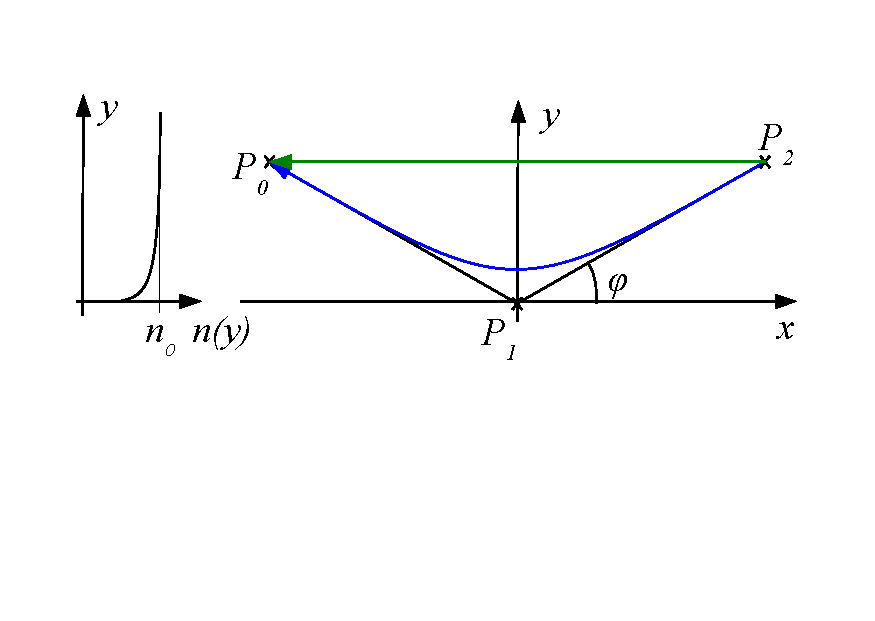
\includegraphics[width=0.8\textwidth]{./picture/FataMorgana.pdf}
	\caption{Skizze der Funktion einer Fata Morgana}
	\label{Ab:fata}
\end{figure}


Wir nehmen an, wir hätten eine Fata Morgana. 
Dabei hat der Brechungsindex die Funktion nach \eqref{brechungsindexFunktion} in Abhängigkeit von $y$ 
(Der Höhe über dem Boden).

\begin{equation}
	n = n_0 (1 - \varepsilon e^{- \alpha y})
	\label{brechungsindexFunktion}
\end{equation}

\texttodo{welcher effekt ist relativ klein?}
Dabei ist der Effekt relativ klein, da $\epsilon << 1$ ist und 
die Skalenlänge $\alpha$ in der Grössenordnung von $\alpha = 1 \cdot m^{-1}$ ist.
Zusätzlich können wir für die Skalierung der x-Richtung die nach \eqref{lichtge} definierte konstante $C$ einführen.

\begin{equation}
	C = n \frac{dx}{ds}
	\label{lichtge}
\end{equation}

Wenn die Strahlengleichung komponentenweise für $r = (y(x), x)$ betrachten wird kann daraus die Strahlengleichung, \eqref{strahlengleichung}, hergeleitet werden.

\begin{equation}
\frac{d}{ds} \left ( n \frac{dy}{ds} \right ) = \frac{d}{dx} \left ( n \frac{dy}{dx} \frac{dx}{ds} \right ) \frac{dx}{ds} =
\frac{d}{dx} \left ( C \frac{dy}{dx} \right ) \frac{C}{n} = \frac{\partial n(y)}{\partial y}
\label{strahlengleichung}
\end{equation}

Da die Konstante $C$ nur die x-Achse skaliert, wird diese auf den Wert $1$ festgelegt.
Wegen 
\texttodo{stimmt diese gleichung? $2 n \partial n / \partial y = \partial n^2 / \partial y$ meiner meinung nach geht da faktor 2 verloren, ist aber schon spät in der Nacht}
\begin{equation}
	2 n \partial n / \partial y = \partial n^2 / \partial y \qquad \text{und} \qquad n^2 \simeq n_0^2(1 - 2 \varepsilon e^{-\alpha y}) \notag
\end{equation}erhalten wir \eqref{difGleich}.

\begin{equation}
	\frac{d^2 y(x)}{dx^2} = \frac{1}{2} \frac{\partial}{\partial y} n^2(y) = n_0^2 \varepsilon \alpha e^{-\alpha y}
	\label{difGleich}
\end{equation}

Diese Gleichung kann mit elementaren Methoden gelöst werden. 
Zudem wird der Steigungswinkel $\varphi$ eingeführt daraus ergibt sich
$\kappa = (\frac{\alpha}{2}) \tan(\varphi)$ daraus ergibt sich die übersichtlichere \eqref{fataFunktion}.
\texttodo{verständlich beschreiben mit zwischen schritten damit sich die diffgleichung und die funktion die gefunden wird ersichtlich sind}
\begin{equation}
	y = y_0 + \frac{1}{\alpha} ln(\cosh^2(\kappa(x - x_0))) \xrightarrow{\kappa (x - x_0 ) >> 1} y =	y_0 + \frac{2 \kappa}{\alpha} (x - x_0)
	\label{fataFunktion}
\end{equation}


In grossen Abständen zum Spiegelpunkt $x_0$ ist die Ausbreitung des Lichtes geradlinig.
Der Beobachter sieht, wie erwarted zwei Bilder, wobei eines auf dem Kopf steht.

\subsection{Lichtwellenleiter}

Hier kommt das vierte Beispiel.